\documentclass[Orbiter User Manual.tex]{subfiles} 
\begin{document}

%TODO update launchpad images
\section{Before you start: The Launchpad}
Starting orbiter.exe brings up the \textit{Orbiter Launchpad} dialog box. The launchpad is your gateway to Orbiter. From here, you can

\begin{itemize}
\item select and launch a simulation scenario
\item set simulation, video and joystick parameters
\item load available plug-in modules to extend the basic Orbiter functionality
\item open the online help system
\item launch the Orbiter simulation window, or
\item exit to the desktop.
\end{itemize}

\noindent
Clicking on one of the tab selector buttons along the left edge of the dialog box opens the corresponding configuration page.

\begin{figure}[H]
	\centering
	\subfigure{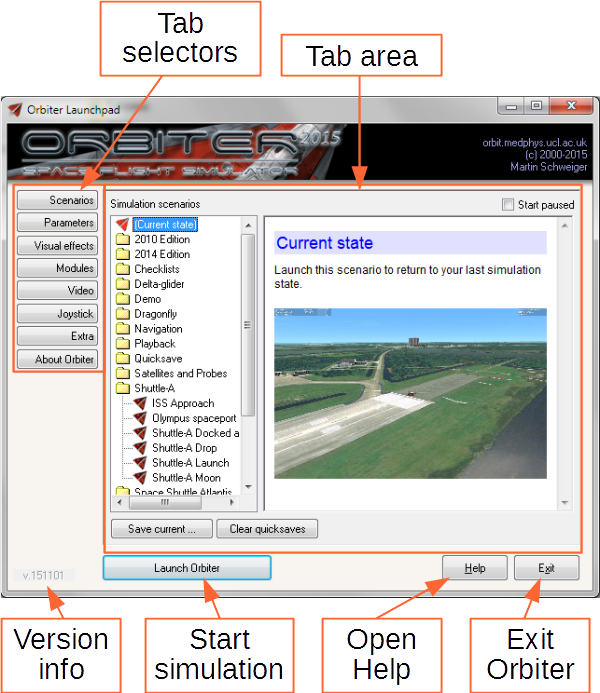
\includegraphics[width=0.65\textwidth]{launchpad.png}}
	\caption{Orbiter Launchpad dialog: Start a simulation scenario, edit parameters and video options, activate modules.}
\end{figure}

\noindent
Important: Before running Orbiter for the first time, make sure that all simulation parameters (in particular the video options) are set correctly.\\
When you are ready, select a scenario and press the "Launch Orbiter" button to jump into the simulation.


\subsection{Scenarios tab}
The \textit{Scenarios} tab allows you to manage and browse the available simulation startup scenarios. A "scenario" defines the initial setup of a simulation session (the date, spacecraft positions, velocities and other parameters).\\
The scenario list contains all stored scenarios (including any you created yourself) in a hierarchical folder structure. Double-click on a folder to open its contents. Double-click on a scenario (marked by the red "Delta-glider" icon) to launch it.\\
Selecting a scenario or folder brings up a description on the right of the dialog box. This can include mission objectives, screenshots and background information.

\begin{figure}[H]
	\centering
	\subfigure{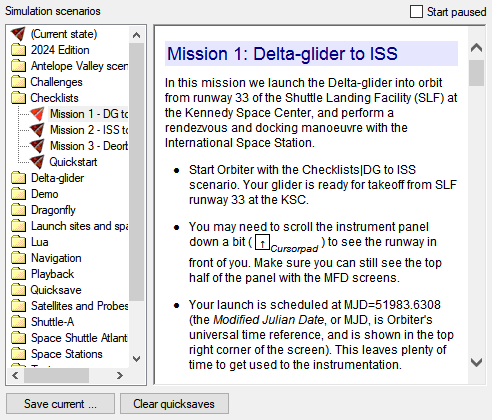
\includegraphics[width=0.65\textwidth]{launchpad_scn.png}}
\end{figure}

\noindent
There are a few special scenarios and folders:

\begin{itemize}
\item The (Current state) scenario is automatically generated whenever you exit the simulator. Use this to continue from the latest exit state.
The Tutorials folder contains pre-recorded flights with on-screen annotations that explain different aspects and stages of spaceflight missions.
\item The Playback folder contains the flights you have recorded with Orbiter’s built-in flight recorder. Launching one of these will start a replay.
\item The Quicksave folder contains in-game saved scenarios generated by pressing \Ctrl\keystroke{S}. Multiple quicksaves are possible. Orbiter saves the quicksave states under the original scenario name, followed by a quicksave counter. The counter is reset each time the simulation is launched, so make sure you copy any scenarios you want to keep!
%TODO add section link
\item The Demo folder can be filled with scenarios that are automatically run in kiosk/demo mode (see Section TODO). This allows to put together a set of simulation runs that can be displayed in unsupervised environments.
\end{itemize}

\noindent
\textbf{To start the simulation paused:}\\
Tick the \textit{Start paused} box to pause the simulation on start. You can resume by pressing \Ctrl\keystroke{P}.\\
\\
\textbf{To save your own scenarios:}\\
%TODO add scenarioeditor link
After exiting a simulation session, click the \textit{Save current} button to save the current simulation state in a new scenario file. For setting up custom simulation scenarios, see also the TODO.\\
\\
\textbf{To clear quicksaved scenarios:}\\
Click the \textit{Clear quicksaves} button to delete all scenarios stored in the Quicksave folder.


\subsection{Parameters tab}
The \textit{Parameters} tab contains various options to customise the simulation behaviour, including realism and difficulty settings, background star rendering, instrument display settings and the focus behaviour for dialog boxes.

\begin{figure}[H]
	\centering
	\subfigure{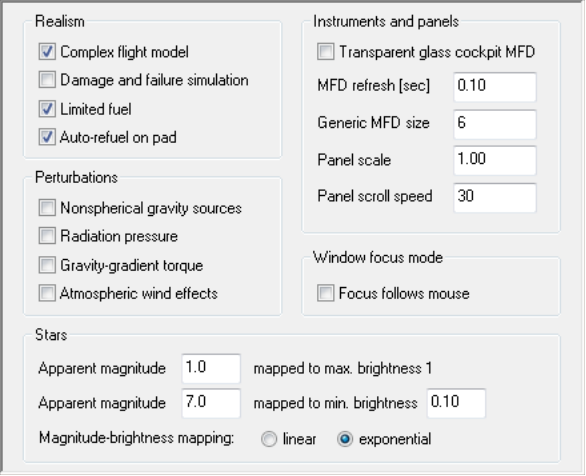
\includegraphics[width=0.65\textwidth]{launchpad_param.png}}
\end{figure}

\noindent
\textbf{Realism}

\begin{itemize}
\item \textbf{Complex flight model:} Select the realism level of the flight model for the spacecraft. Tick this box to enable the most realistic flight parameters available for all vessel types. Disabling this option may activate simplified flight parameters which make spacecraft easier to control for newcomers. Not all vessel types may support this option.
\item \textbf{Damage and failure simulation:} Spacecraft can sustain damage and system failure, for example if operational limits are exceeded. Not all vessel types may support this option.
\item \textbf{Limited fuel:} Untick this box to ignore fuel consumption of your spacecraft.
\alertbox{Some of the more "realistic" spacecraft, such as the Space Shuttle, may not work properly if "Limited fuel" is not selected, because they rely on the reduction of mass during lift-off as a consequence of fuel consumption.}
%TODO add tech note link
\item \textbf{Nonspherical gravity sources:} This option activates a more complex gravity force calculation which can take into account perturbations in the gravitational potential due to non spherical celestial body shapes, thus allowing more accurate orbit predictions. Note that this option can make orbital calculations more difficult, and may reduce the reliability of instruments that don’t take this effect into account. For a planet to make use of the perturbation code, its configuration file must supply shape parameters via the \textit{JCoeff} entry. For background and technical implementation details please refer to TODO.
%TODO add tech note link
\item \textbf{Gravity-gradient torque:} If this option is enabled, vessels can experience an angular moment in the presence of a gravitational field gradient. This will be noticeable in particular in low orbits and can lead to attitude oscillations around the equilibrium or attitude-locked orbits. For background and technical implementation details please refer to TODO.
\end{itemize}

\noindent
\textbf{Window focus mode}

\begin{itemize}
\item Focus follows mouse: If this option is ticked, the input focus is automatically switched to the window under the mouse pointer. If unticked, the focus is switched in normal Windows style by clicking the window.
\end{itemize}

\noindent
\textbf{Instruments}

\begin{itemize}
%TODO add section link
\item \textbf{Transparent MFD:} Make the multifunctional displays in glass cockpit mode (see Sec. TODO) transparent. This provides a better view of the 3-D environment, but makes it more difficult to read the instruments.
\item \textbf{MFD refresh:} Time (in seconds) between MFD updates. Shorter intervals provide smoother updates, but may degrade performance. Some built-in MFD modes, such as the Surface and HSI modes, override the user-defined update frequency.
\item \textbf{Panel scale:} Sizing factor for instrument panels. Scale 1 provides optimal visual quality, but other values may be used to adapt the panel size at low or high screen resolutions.
\item \textbf{Panel scroll speed:} Determines how fast the panel can be scrolled across the screen [pixels/second]. Negative values invert the panel scroll directions.
\end{itemize}


\subsection{Visual effects tab}
The \textit{Visual effects} tab provides options for tuning the rendering parameters and graphic detail. These options will improve the visual appearance and realism of the simulator, but most of them can have an adverse effect on simulation performance (frame rates) when enabled, and may increase video and main memory demands, so they should be used with care, in particular on less powerful computers. As a first step in troubleshooting Orbiter problems it is often a good idea to turn off all visual effects.

\begin{figure}[H]
	\centering
	\subfigure{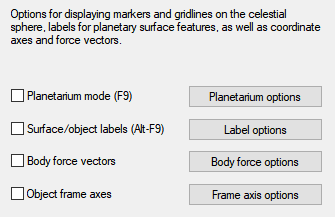
\includegraphics[width=0.65\textwidth]{launchpad_visual.png}}
\end{figure}

\noindent
Note that some advanced rendering options can also be found in the \textit{Extra} tab, under \textit{Visualisation parameters}. This includes mip­map and anisotropic filtering options as well as texture and elevation resolution bias settings.\\
\\
\textbf{Planetary effects}

\begin{itemize}
\item \textbf{Cloud layers:} Add a cloud layer above the surface for planets which support it.

\begin{figure}[H]
	\centering
	\subfigure{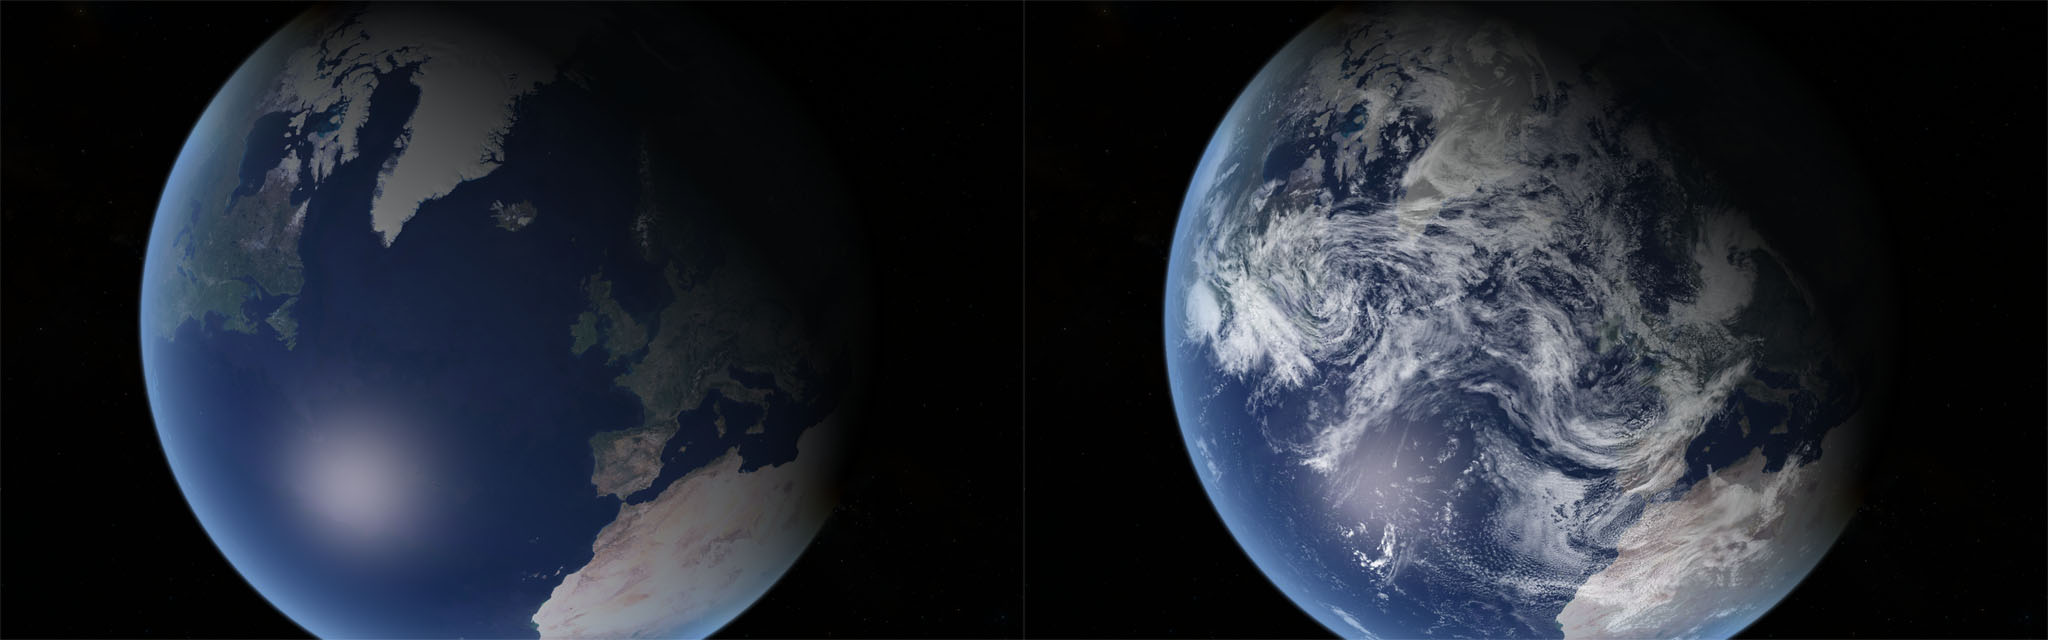
\includegraphics[width=0.95\textwidth]{planet_clouds.png}}
	\caption{Cloud layers disabled (left) and enabled (right).}
\end{figure}

\item \textbf{Cloud shadows:} Render cloud shadows cast on the planet surface. Only planets whose config files contain a CloudShadowDepth entry < 1 will actually render cloud shadows.

\begin{figure}[H]
	\centering
	\subfigure{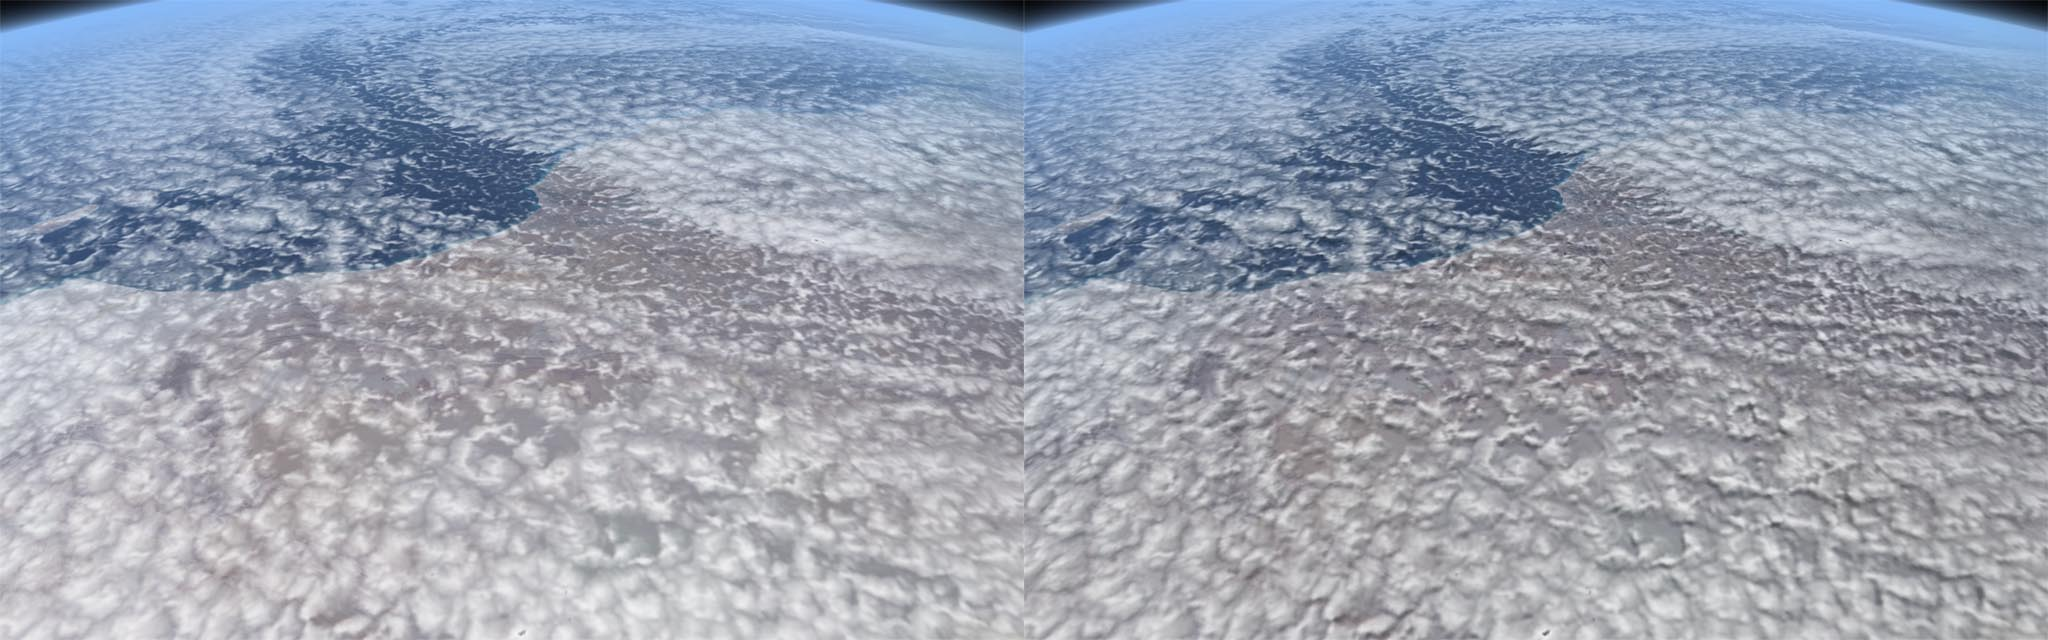
\includegraphics[width=0.95\textwidth]{planet_cloud_shadows.png}}
	\caption{Cloud shadows disabled (left) and enabled (right).}
\end{figure}

\item \textbf{Horizon haze:} Render an intensity-graded ("glowing") horizon layer for planets with atmospheres.

\begin{figure}[H]
	\centering
	\subfigure{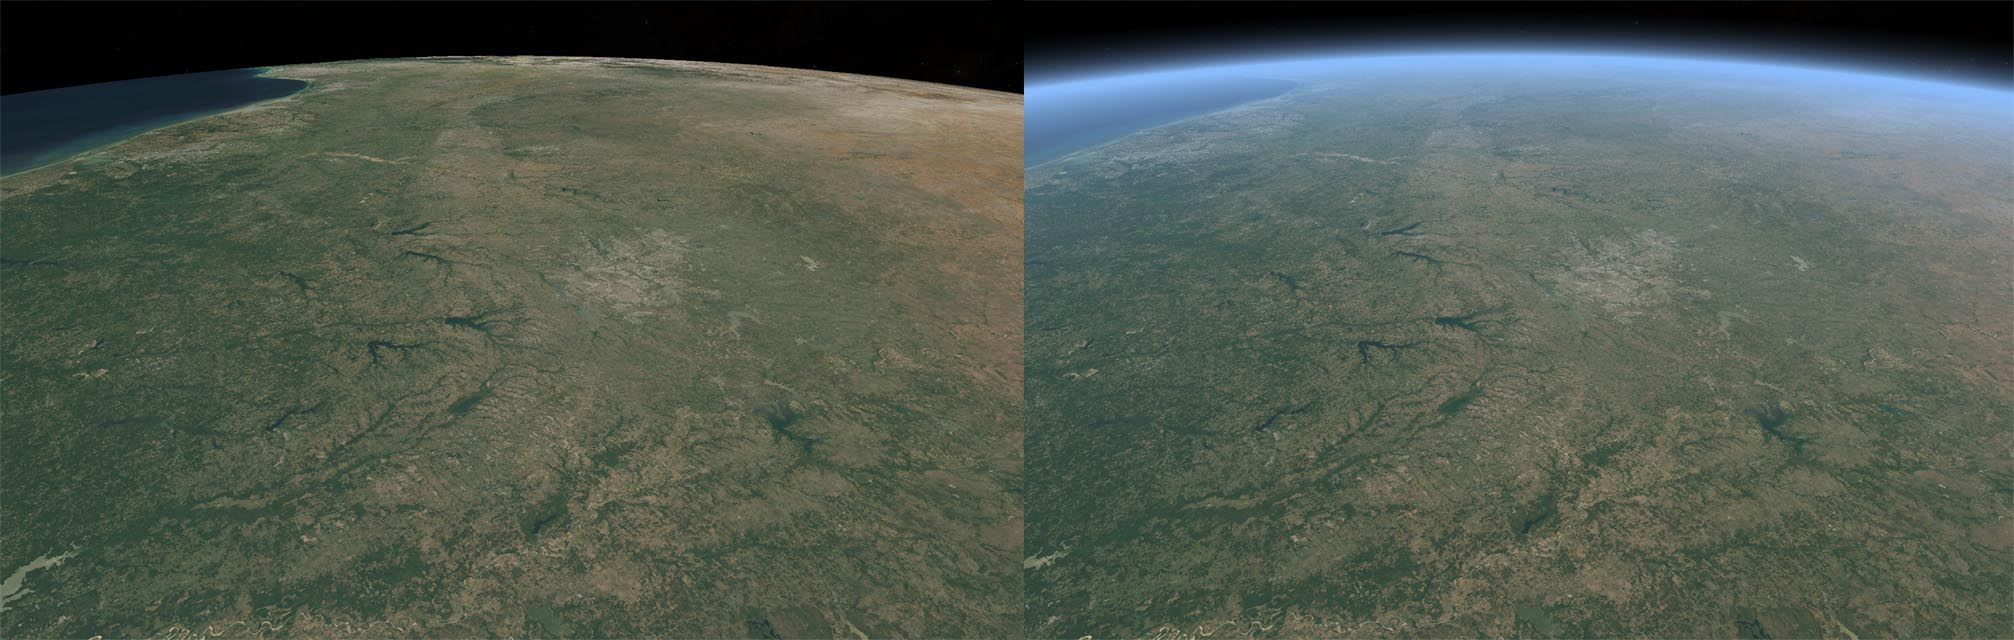
\includegraphics[width=0.95\textwidth]{planet_haze.png}}
	\caption{Horizon haze disabled (left) and enabled (right).}
\end{figure}

\item \textbf{Distance fog:} Apply atmospheric mist and fog effects to distant objects when viewed through planetary atmospheres.

\begin{figure}[H]
	\centering
	\subfigure{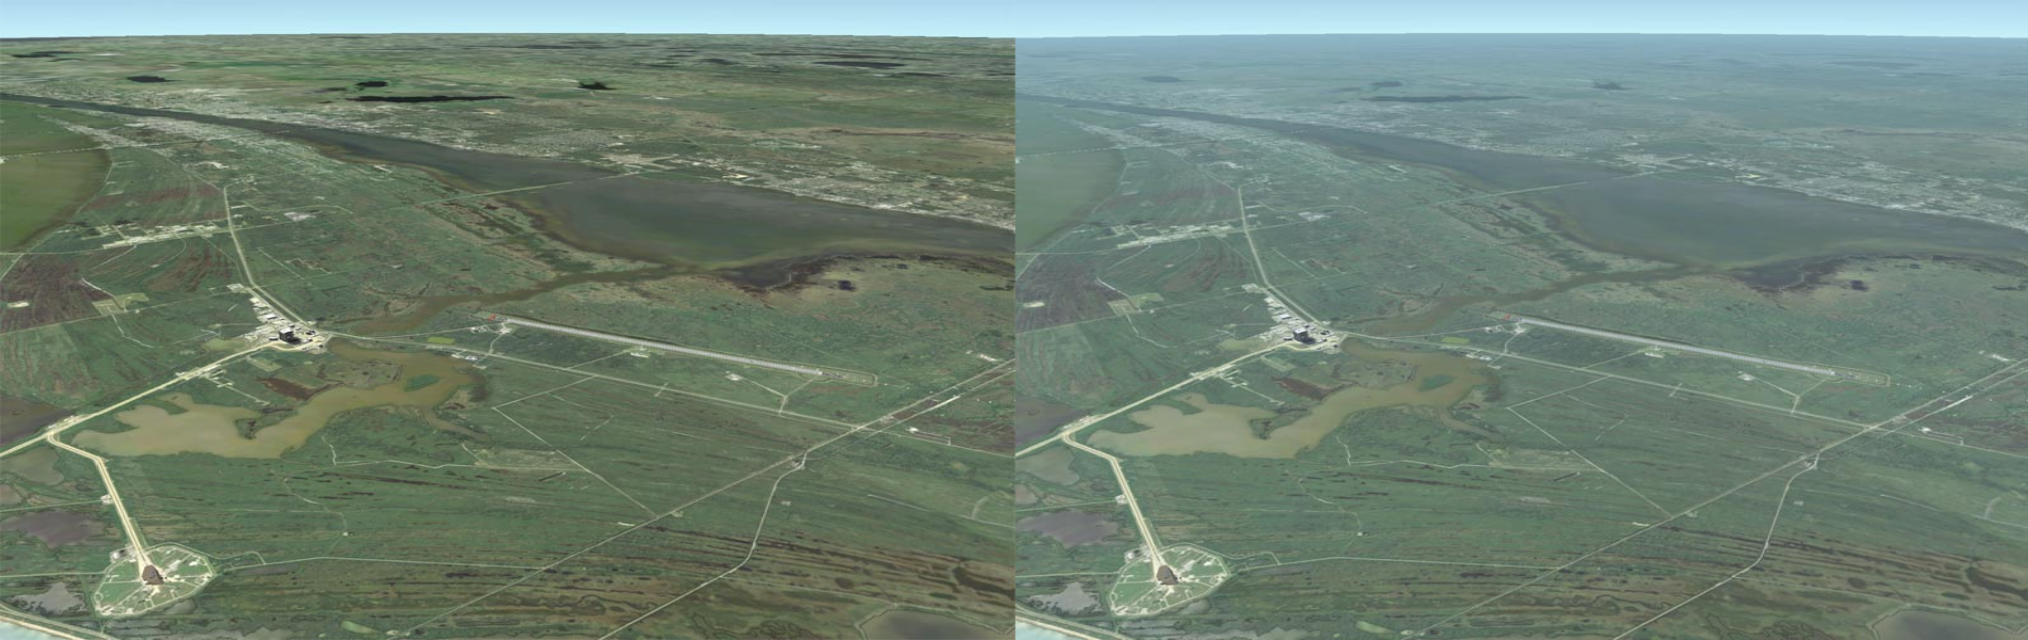
\includegraphics[width=0.95\textwidth]{planet_fog.png}}
	\caption{Distance fog disabled (left) and enabled (right).}
\end{figure}

\item \textbf{Specular water reflections:} Render water surfaces on planets with specular reflection effects.

\begin{figure}[H]
	\centering
	\subfigure{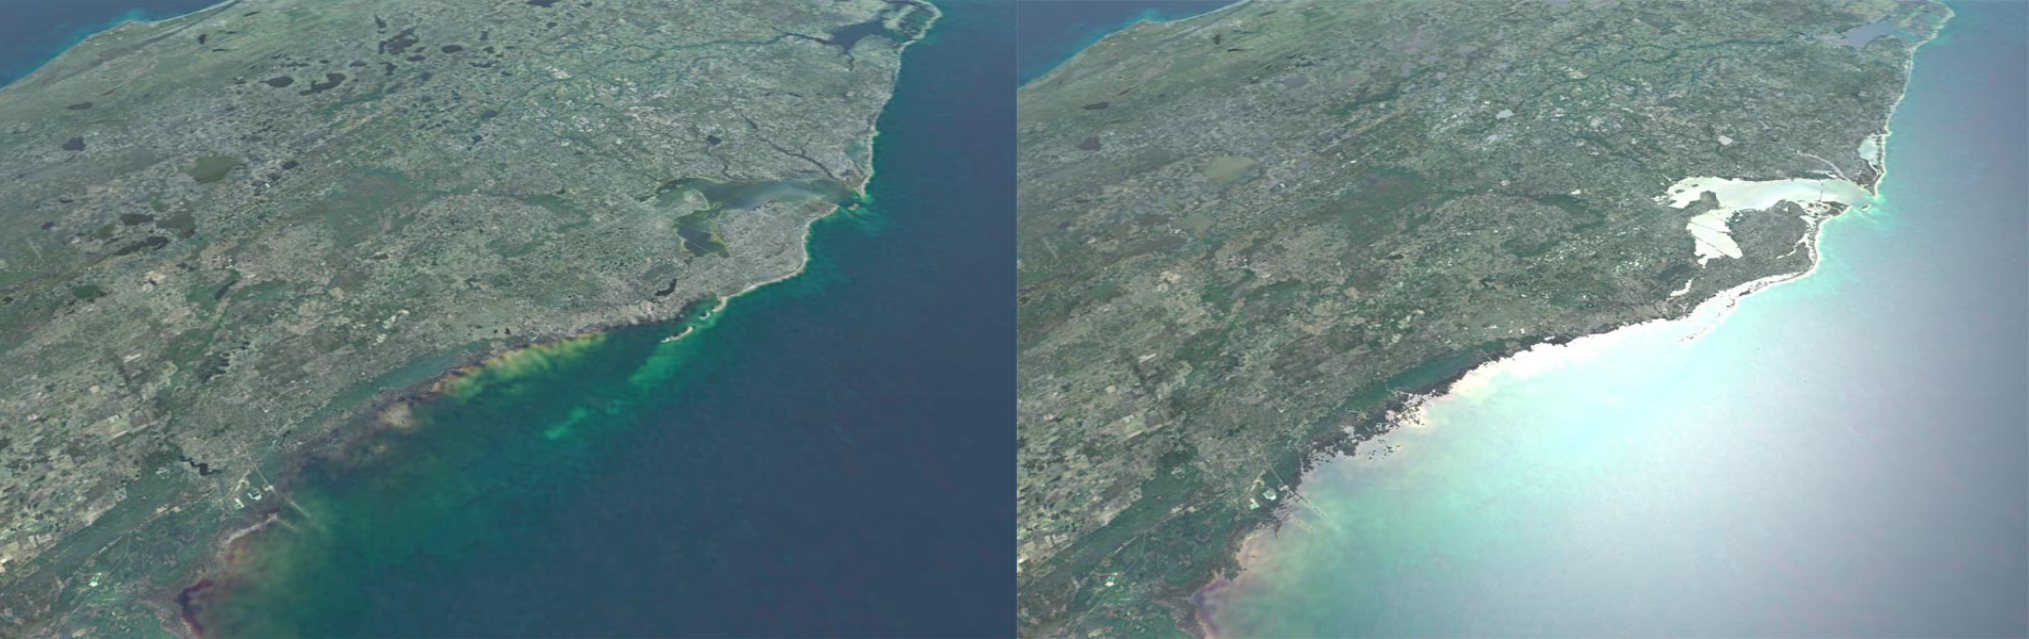
\includegraphics[width=0.95\textwidth]{planet_water.png}}
	\caption{Specular water reflections disabled (left) and enabled (right).}
\end{figure}

\item \textbf{Specular ripples:} Generate "ripple" effect in specular reflections from oceans for improved appearance of water surfaces.

\begin{figure}[H]
	\centering
	\subfigure{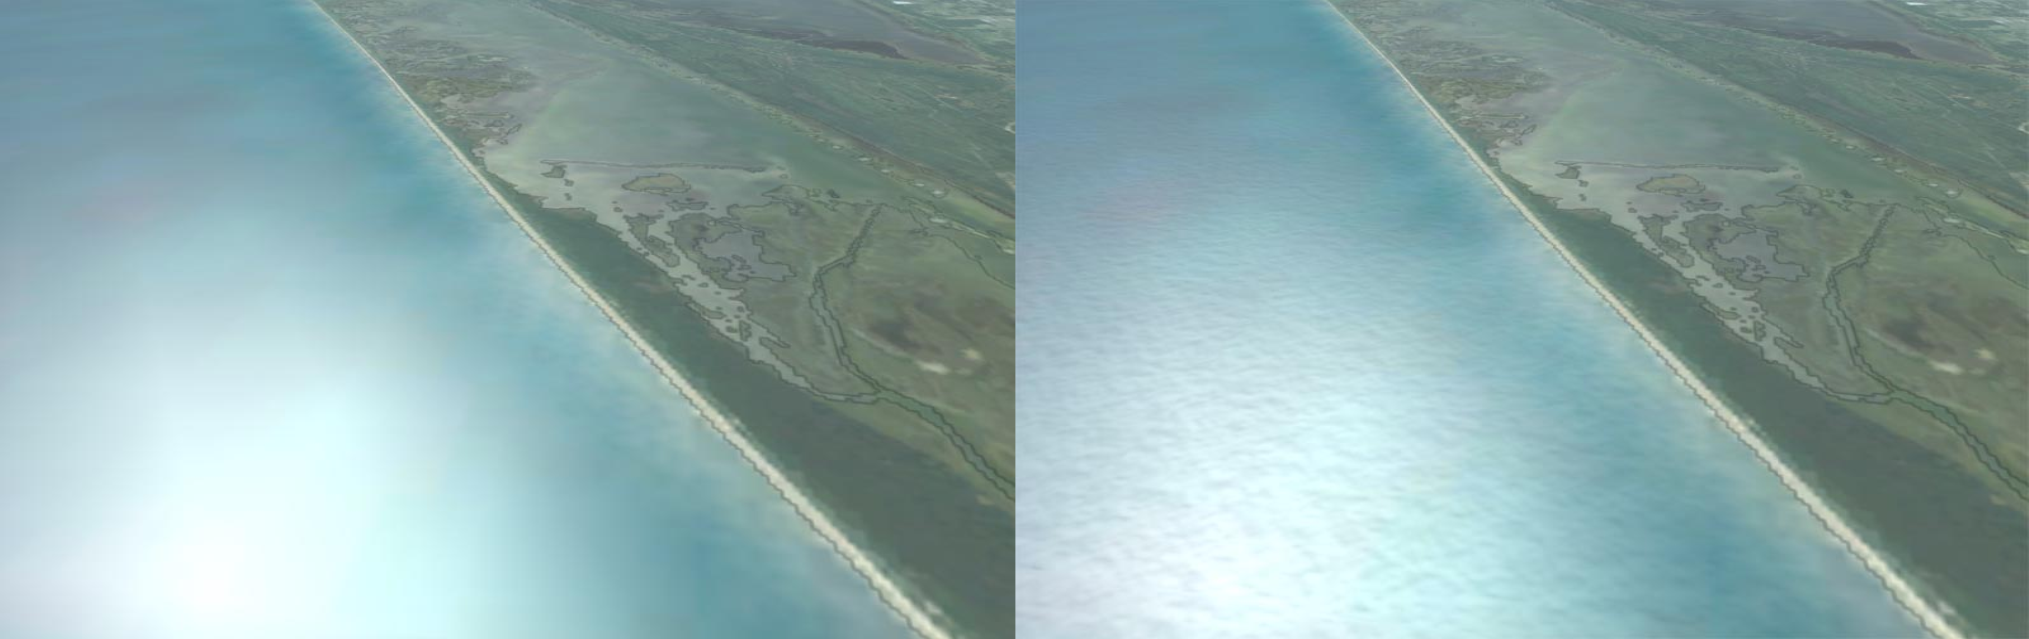
\includegraphics[width=0.95\textwidth]{planet_specular.png}}
	\caption{Specular ripples disabled (left) and enabled (right).}
\end{figure}

\item \textbf{Planet night lights:} Render city lights during night-time where available.

\begin{figure}[H]
	\centering
	\subfigure{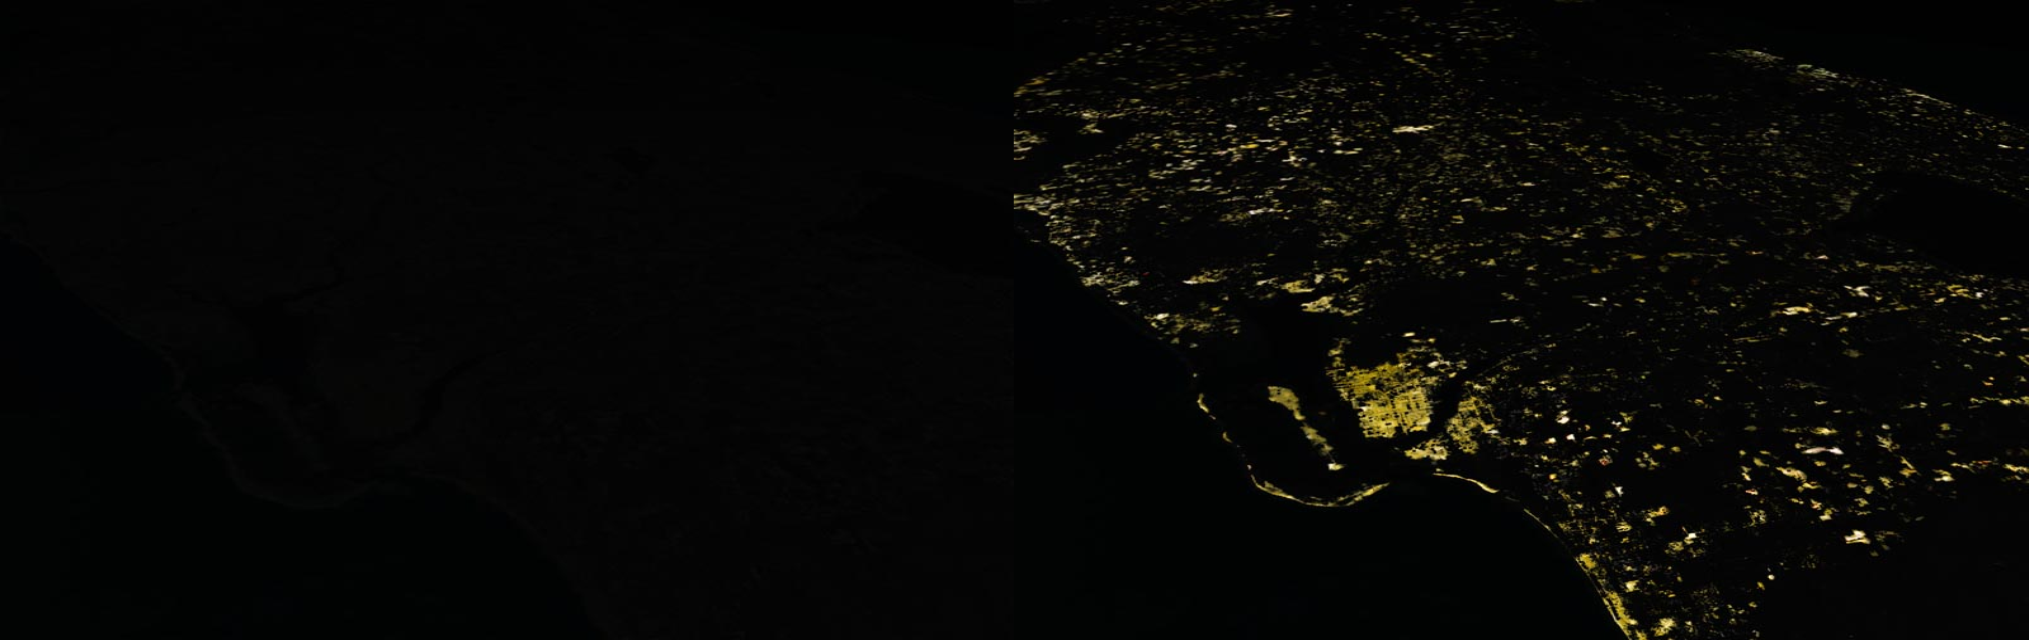
\includegraphics[width=0.95\textwidth]{planet_night.png}}
	\caption{Planet night lights disabled (left) and enabled (right).}
\end{figure}

\item \textbf{Night light level:} Defines the brightness of night city lights. Valid range is 0 to 1 (ignored if planet night lights are disabled).
\item \textbf{Surface elevation:} Enable or disable modelling of ground elevation on planetary surfaces. When enabled, select between linear and cubic (smoother) interpolation of elevation data.

\begin{figure}[H]
	\centering
	\subfigure{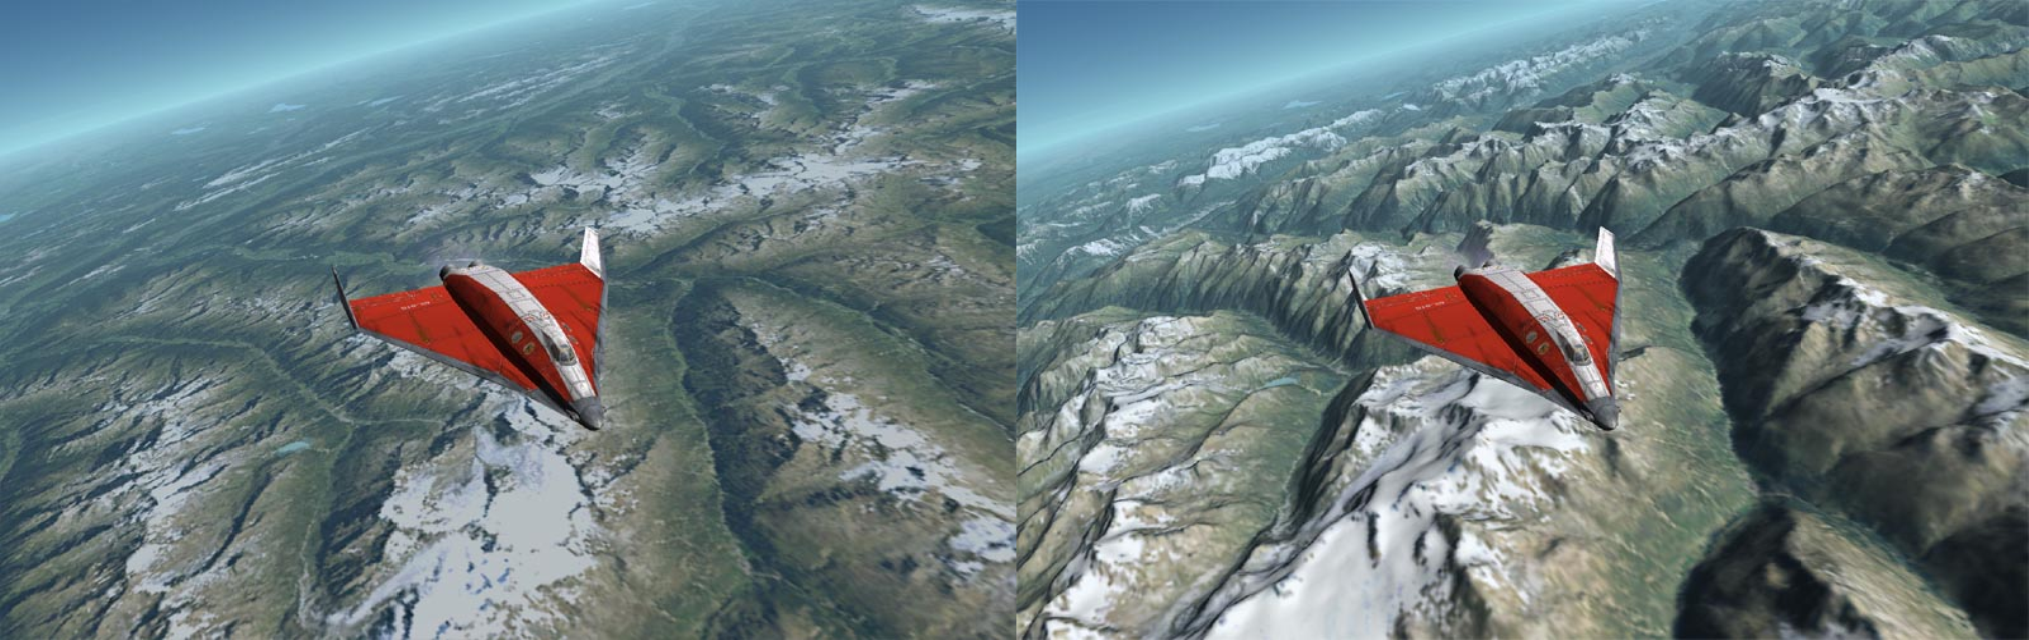
\includegraphics[width=0.95\textwidth]{planet_elevation.png}}
	\caption{Planet surface elevation disabled (left) and enabled (right).}
\end{figure}

\item \textbf{Max. resolution level:} The maximum resolution at which planetary surfaces can be rendered. Supported values are 1 to 19. Higher values provide better visual appearance of planets that support high texture resolutions, but also significantly increase the demand on computing resources (graphics processor and memory). Note that the actual resolution level supported by any planetary body may be lower than this value, depending on the texture set available. Higher resolution textures for many bodies may be downloaded from the Orbiter website or add-on repositories. The highest resolution levels are usually only supported in selected areas on the surface (e.g. around spaceports).

\begin{figure}[H]
	\centering
	\subfigure{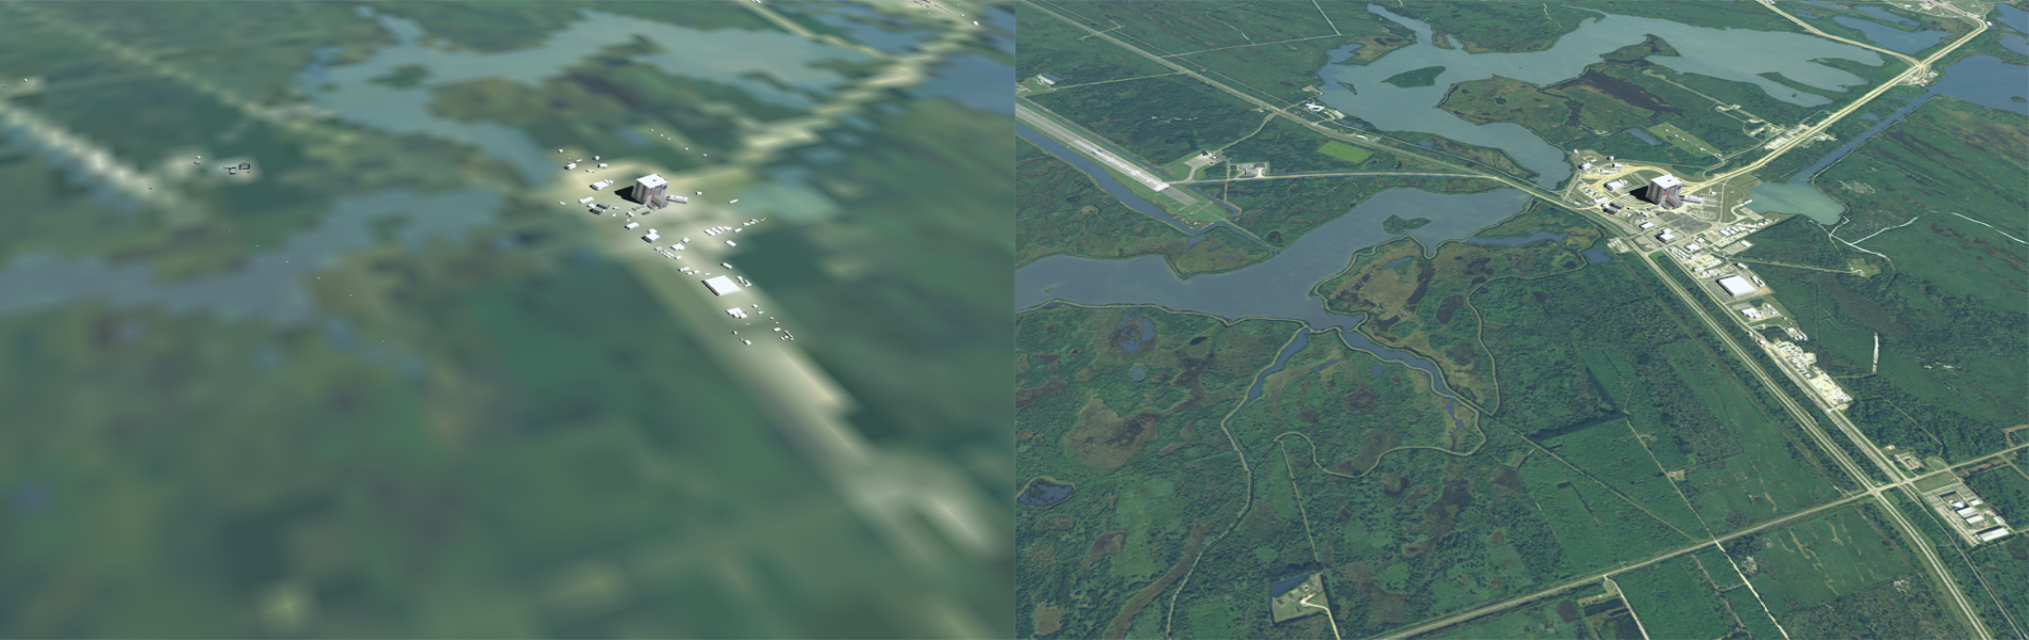
\includegraphics[width=0.95\textwidth]{planet_tile_res.png}}
	\caption{Kennedy Space Center at resolution level 12 (left) and 19 (right)}
\end{figure}

\end{itemize}

\noindent
\\
\textbf{General effects}

\begin{itemize}
\item \textbf{Vessel shadows:} Enable shadows cast by spacecraft on planet surfaces.
\item \textbf{Object shadows:} Enable dynamic shadows of ground-based objects such as buildings.
\item \textbf{Specular reflection from objects:} Render reflective surfaces like solar panels, window panes and metallic surfaces. May degrade performance.
\item \textbf{Reentry flames:} Render a glowing plasma hull during reentry.
\item \textbf{Particle streams:} Render ionised exhaust gases and vapour trails with particle effects.
\item \textbf{Local light sources:} Enable localised light sources, e.g. from engines, landing lights, floodlights etc. This option can have a significant influence on frame rates.
\item \textbf{Ambient light level:} Defines the brightness of the unlit side of planets and moons. Ambient level 0 is the most realistic, but makes it difficult to spot objects in the dark. Level 255 is uniform lighting (no darkness).
\end{itemize}


\subsection{Modules tab}
The \textit{Modules} tab allows the activation and deactivation of plug-in modules for Orbiter which can extend the functionality of the core simulator. Plug-ins can contain additional instruments, dialogs, interfaces to external programs etc. Make sure you only activate modules you actually want to use, because modules can take up some processing time even if they run in the background, and thus affect Orbiter’s performance.

\begin{figure}[H]
	\centering
	\subfigure{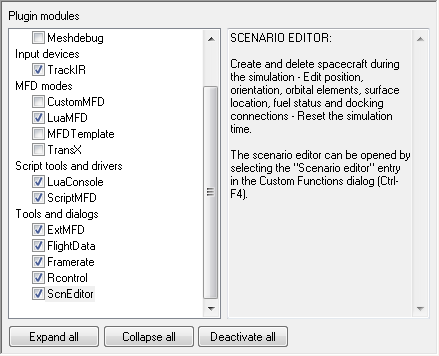
\includegraphics[width=0.65\textwidth]{launchpad_modules.png}}
\end{figure}

\noindent
To activate a module, click the tick box next to its entry in the list. By clicking on the entry itself, many modules provide a short description about their function and user interface in the right panel. Entries are grouped in categories. You can expand or collapse categories by double-clicking the category header. The buttons at the bottom of the tab allow expanding or collapsing the entire list, and quick deactivation of all modules.\\
The modules provided with the standard Orbiter distribution are demos from the SDK package, and are available in full source code. A wide variety of additional modules by 3$^{rd}$ party add-on developers can be downloaded from Orbiter repositories on the internet.\\
Some of the standard modules distributed with Orbiter are:

\begin{itemize}
%TODO add section link
\item \textbf{ScnEditor:} A versatile scenario editor that allows adding, editing and deleting spacecraft in a running simulation. See Section TODO for more details.
\item \textbf{ExtMFD:} This module allows to open additional multifunctional displays in external dialog boxes. Useful if you need more information than a vessel’s built-in MFD displays provide, or if you want to track flight data in external camera views.
\item \textbf{CustomMFD:} This module provides an additional Ascent MFD mode for the multifunctional displays, which can be selected via \Shift\keystroke{F1}-\Shift\keystroke{P}. The sources for this module are a good starting point for developers who want to create their own MFD modes.
\item \textbf{Rcontrol:} Remote control of ship engines. This allows to manipulate vessels even if they don’t have input focus. If this module is active, the remote control window can be selected from the Custom Functions list (\Ctrl\keystroke{F4}).
\item \textbf{FlightData:} Real-time atmospheric flight data telemetry. If this module is active, the flight data window can be selected from the \textit{Custom Functions} list (\Ctrl\keystroke{F4}).
\item \textbf{Framerate:} A graphical simulation frame rate (FPS) display. If this module is active, the frame rate window can be selected from the \textit{Custom Functions} list (\Ctrl\keystroke{F4}).
\item \textbf{LuaConsole:} Provides a console window for interactive processing of script commands. Can be opened via the \textit{Custom Functions} list.
\item \textbf{LuaMFD:} Adds a new MFD mode for script input via a console MFD.
\end{itemize}


\subsection{Video tab}
The \textit{Video} tab provides options to select the rendering device, switch between full-screen and windowed mode, and set the resolution, window size and colour depth.

\begin{figure}[H]
	\centering
	\subfigure{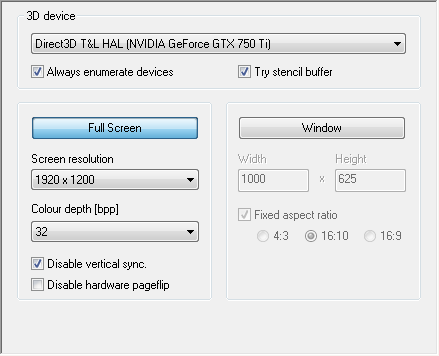
\includegraphics[width=0.65\textwidth]{launchpad_video.png}}
\end{figure}

\noindent

\begin{itemize}
\item \textbf{3D Device:} Lists the available hardware and software devices for 3-D rendering. Select a hardware device with transform and lighting capabilities when possible, such as \textit{Direct3D T\&L HAL} or similar. (On some systems, the hardware devices might be listed with the name of your graphics card). Software devices such as \textit{RGB Emulation} will provide poor performance or not run at all. Note that some older hardware devices do not support window mode.
%TODO switch italics below to alertbox or such?
\item \textbf{Always enumerate devices:} Tick this box if Orbiter does not display 3D devices or screen modes correctly. This option enforces a hardware scan whenever Orbiter is launched and skips the device data stored in device.dat. \textit{Make sure you tick this box after upgrading your graphics hardware or DirectX/video drivers to make Orbiter aware of the changes.}
\item \textbf{Try stencil buffer:} Enables stencil buffering, if the video mode supports it. Stencil buffers can improve various visual effects (for example, provide support for alpha-blended shadows), but may have a slight impact on frame rates. If the selected video mode doesn’t support stencil buffers, this option is ignored.
\item \textbf{Full screen:} Select this option to run Orbiter in full-screen mode. You can choose the screen resolution and colour depth from the list provided. Only modes supported by the selected device are listed here. Higher resolution and colour depth will improve the visual appearance at the cost of reduced performance. Note that selecting a low colour depth can lead to visual artefacts (insufficient depth resolution).\newline
In addition, you can select the \textit{Disable vertical sync} option. This allows Orbiter to update a frame without waiting for a synchronisation signal from the monitor. This can improve frame rates, but may lead to visual artefacts (tearing).\newline
On some systems the hardware frame buffer switching may cause the screen occasionally to flash white. Use \textit{Disable hardware pageflip} to solve this problem. Disabling hardware pageflip also disables vertical sync.
\item \textbf{Window:} Select this option to run Orbiter in a window. You can specify the size of the render window here. Selecting one of the available \textit{fixed aspect ratio} options (4:3 normal, 16:10 widescreen or 16:9 widescreen) automatically adjusts the window width or height to maintain the aspect ratio. Large window sizes can reduce simulation performance. Note that some older graphics drivers may not allow 3-D applications to run in window mode.
\end{itemize}


\subsection{Joystick tab}
The \textit{Joystick} tab allows selection and configuration of your joystick device, if present.

\begin{figure}[H]
	\centering
	\subfigure{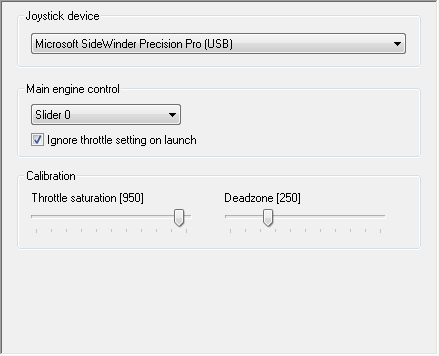
\includegraphics[width=0.65\textwidth]{launchpad_joystick.png}}
\end{figure}

\noindent

\begin{itemize}
\item \textbf{Joystick device:} Lists all attached joysticks.
\item \textbf{Main engine control:} Define the joystick axis which controls the main thrusters. Try different options if the throttle control on your joystick doesn’t work in Orbiter.\newline
Ignore throttle setting on launch: If ticked, the joystick throttle will be ignored at the launch of a scenario until the user manipulates it. Otherwise, the throttle setting is used immediately.
\item \textbf{Deadzone:} Use this to define how soon the joystick will respond when moved out of its centre position. Smaller values make it respond sooner. Increase if attitude thrusters do not cut out completely in neutral position.
\item \textbf{Throttle saturation:} Defines the tolerance zone at the minimum and maximum range of the throttle control at which the joystick reports zero and maximum throttle, respectively. Reduce if main engines do not cut out completely at minimum throttle setting. (Applies only to joysticks with throttle control).
\end{itemize}

\noindent
If further calibration is required you should use the appropriate tools in the Windows Control Panel.


\subsection{Extra tab}
The \textit{Extra} tab contains a list of more advanced and specialised settings and configuration parameters, including details about Orbiter’s dynamic state propagation, vessel configuration and debugging options. Add-on plug-ins may add their own configuration entries to the list when activated.

\begin{figure}[H]
	\centering
	\subfigure{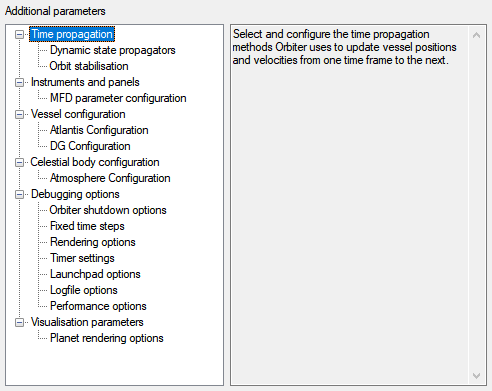
\includegraphics[width=0.65\textwidth]{launchpad_extra.png}}
\end{figure}

\noindent
It is generally safe for new users to leave all settings in this list at their default values. Advanced users can fine-tune the behaviour of the simulator here.\\
Click on an item to see a short description of its purpose to the right of the list. Double-clicking, or pressing the \textit{Edit} button opens the associated configuration dialog. Among the default configuration options available are:

\begin{itemize}
%TODO add tech ref link
\item \textbf{Time propagation:} defines the parameters for dynamic update of linear (position and velocity) and angular vessel states (orientation and angular velocity). Users can select the integration methods as a function of step interval. The \textit{Orbit stabilisation} entry allows to configure the conditions under which Orbiter switches from dynamic to orbit perturbation updates. For technical details on the dynamic propagation schemes available in Orbiter, refer to TODO.
\item \textbf{Vessel configuration:} Different spacecraft types may provide options for defining visual and physical behaviour under this section.
\item \textbf{Celestial body configuration:} Parameters to define particular characteristics of planetary bodies. Currently this section contains configuration options for the atmospheric models of some planets.
\item \textbf{Debugging options:} Miscellaneous settings, including the way Orbiter shuts down a simulation session and the option to enforce fixed time steps, which can be useful for debugging or trajectory generation.
\item \textbf{Visual parameters:} This section contains advanced rendering and texture load options for planetary bodies.
\end{itemize}


\subsection{About Orbiter tab}
The \textit{About Orbiter} tab contains version and build information, as well as links to the Terms of Use, credits and the Orbiter home page and forum.

\begin{figure}[H]
	\centering
	\subfigure{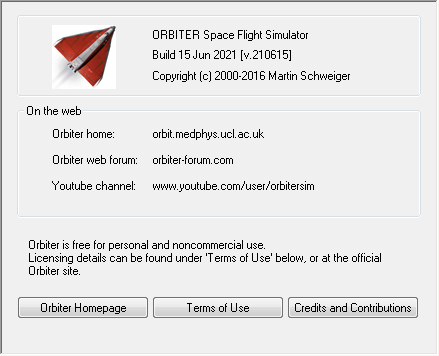
\includegraphics[width=0.65\textwidth]{launchpad_about.png}}
\end{figure}

\end{document}
